\newpage
\section{Description of Models}
\todo[inline]{This section shall describe your models for the different subsystems for the two architectures and the two levels of functionality. Figures should be explained in the text.}

%\Tree[.{WU Failure} [.{$1 \geq$} [.{CM subsystem fail} [.{\&} {CM1 fail} {CM2 fail} ] ] [.{S subsystem fail} [.{\&} {S1 fail} {S2 fail} ] ] [.{A subsystem fail} {A fail} ] ] ] 

\subsection{Wheel Unit Model}
\begin{figure}[H]
  \centering
  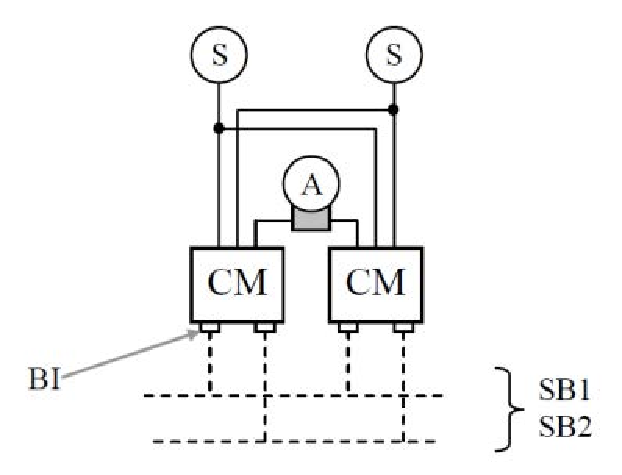
\includegraphics[scale=0.7]{Fig2.pdf}
  \caption{Wheel Unit}
  \label{fig2}
\end{figure}
\begin{figure}[H]
  \centering
  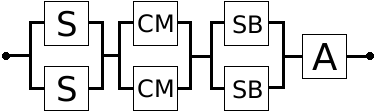
\includegraphics[scale=1]{wu_block.png}
  \caption{Reliability block diagram of the wheel unit}
  \label{fig3}
\end{figure}
%--------------------------------
\subsection{Wheel Unit Subsystem Model}
/text/
\begin{figure}[H]
  \centering
  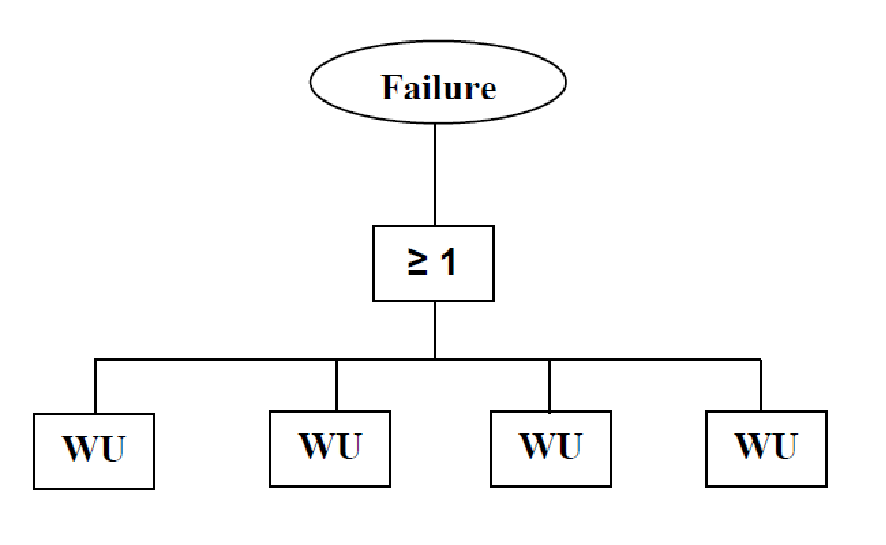
\includegraphics[scale=0.5]{Fig4.pdf}
  \caption{Fault tree for the Wheel Unit Subsystem, full functionality}
  \label{fig4}
\end{figure}
\begin{figure}[H]
  \centering
  %
\includegraphics[scale=0.5]{Fig5.pdf}
  \Tree[.{WU Failure} [.{$2 \geq$} WU WU WU WU ] ]
  \caption{Fault tree for the Wheel Unit Subsystem, degraded functionality}
  \label{fig5}
\end{figure}
%--------------------------------
\subsection{Central Unit (CU)}
\subsubsection{Distributed Duplex Architecture}
\begin{figure}[H]
  \centering
  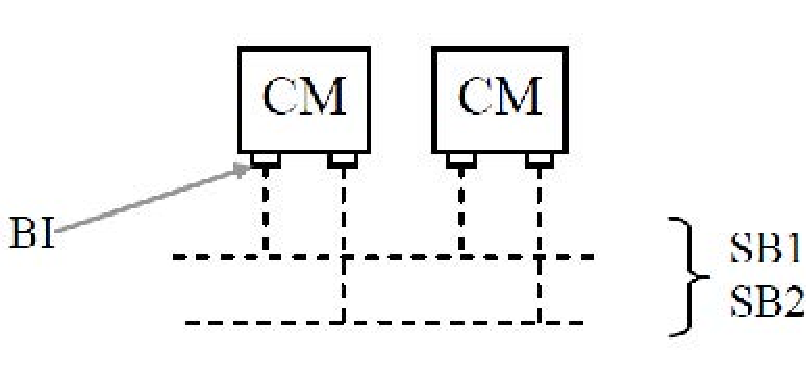
\includegraphics[scale=.5]{Fig6.pdf}
  \caption{Central Unit, duplex configuration }
  \label{fig6}
\end{figure}
\begin{figure}[H]
  \centering
  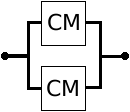
\includegraphics[scale=.5]{cm2_block.png}
  \caption{Reliability block diagram for the Central Unit, duplex configuration}
  \label{fig7}
\end{figure}
%The markov model for central unit-duplex is given below as an example. 
%\begin{figure}[h!]
%  \centering
%  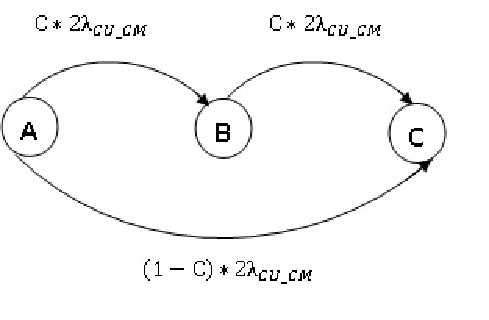
\includegraphics[scale=.7]{Fig8.pdf}
%  \caption{Markov model for the Central Unit. duplex configuration}
%  \label{fig8}
%\end{figure}
\begin{figure}[h!]
\begin{center}
\begin{tikzpicture}[node distance=5mm and 20mm]
\node[state] (s2) {A};
\node[state] (s3) [right= of s2] {B};
\node[state] (s4) [right= of s3] {C};
\draw [->,bend left=45] (s2) to node[above] {$c*2\lambda_{CU-CM} $} (s3);
\draw [->,bend right=45] (s2) to node[above] {$(1-c)*2\lambda_{CU-CM}$} (s4);
\draw [->,bend left=45] (s3) to node[above] {$\lambda_{CU-CM}$} (s4);
\end{tikzpicture}
\caption{Markov chain model}
\end{center}
\end{figure}
%-------------
\subsubsection{Centralized Triplex Architecture}

\begin{figure}[H]
  \centering
  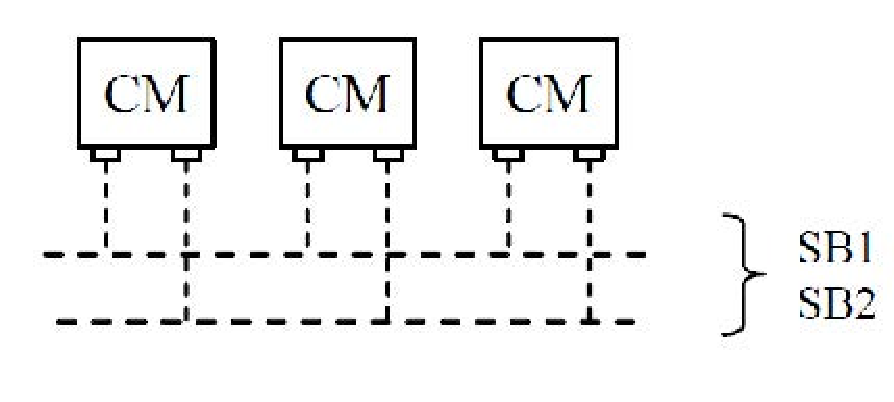
\includegraphics[scale=.5]{Fig9.pdf}
  \caption{Central Unit, triplex configuration }
  \label{fig9}
\end{figure}
/{Reliability block diagram for …, Figure 10.  Make sure the caption number is correct.}/
\\/{Markov model for …, Figure 11.}/

\begin{figure}[H]
  \centering
  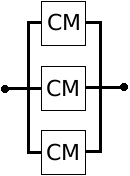
\includegraphics[scale=.5]{cm3_block.png}
  \caption{Caption }
  \label{fig10}
\end{figure}
\begin{figure}[H]
  \centering
  %
\includegraphics[scale=.5]{Fig11.pdf}
  \begin{tikzpicture}[node distance=5mm and 20mm]
    \node[state] (sa) {A};
    \node[state] (sb) [right= of s2] {B};
    \node[state] (sc) [right= of s3] {C};
    \draw [->,bend left=45] (s2) to node[above] {$c*2\lambda_{CU-CM} $} (s3);
    \draw [->,bend right=45] (s2) to node[above] {$(1-c)*2\lambda_{CU-CM}$} (s4);
    \draw [->,bend left=45] (s3) to node[above] {$\lambda_{CU-CM}$} (s4);
  \end{tikzpicture}
  \caption{Caption}
  \label{fig11}
\end{figure}
%--------------------------------
\subsection{System Model}
\subsubsection{Centralized Architecture}

\begin{figure}[H]
  \centering
  %
\includegraphics[scale=.5]{Fig12.pdf}
  \Tree[.{System Failure} [.{$1 \geq$} [.{CU subsystem fail} [.{$2 \geq$} CM CM CM ] ] [.{WU subsystem fail} [.{$1 \geq$} WU WU WU WU ] ] [.{SB subsystem fail} [.{\&} SB SB ] ] ] ]
  \caption{Fault tree for Full Functionality}
  \label{fig12}
\end{figure}
\begin{figure}[H]
  \centering
  %
\includegraphics[scale=.5]{Fig13.pdf}
  \Tree[.{System Failure} [.{$1 \geq$} [.{CU subsystem fail} [.{$2 \geq$} CM CM CM ] ] [.{WU subsystem fail} [.{$2 \geq$} WU WU WU WU ] ] [.{SB subsystem fail} [.{\&} SB SB ] ] ] ]
  \caption{Fault tree for Degraded Functionality}
  \label{fig13}
\end{figure}
%-------------
\subsubsection{Distributed Architecture}
\begin{figure}[H]
  \centering
  %
\includegraphics[scale=.5]{Fig14.pdf}
  \Tree[.{System Failure} [.{$1 \geq$} [.{CU subsystem fail} [.{$1 \geq$} CM CM ] ] [.{WU subsystem fail} [.{$1 \geq$} WU WU WU WU ] ] [.{SB subsystem fail} [.{\&} SB SB ] ] ] ]
  \caption{Fault tree for Full Functionality}
  \label{fig14}
\end{figure}
\begin{figure}[H]
  \centering
  %
\includegraphics[scale=.5]{Fig15.pdf}
  \Tree[.{System Failure} [.{$1 \geq$} [.{CU subsystem fail} [.{$1 \geq$} CM CM ] ] [.{WU subsystem fail} [.{$2 \geq$} WU WU WU WU ] ] [.{SB subsystem fail} [.{\&} SB SB ] ] ] ]
  \caption{Fault tree for Degraded Functionality}
  \label{fig15}
\end{figure}